\subsection{Evaluation Metrics}
We designed the following metrics to evaluate both teacher and student policy performance.
Let $\tau\in\{1,\dots,N\}$ index evaluation episodes and $t\in\{0,\dots,T_\tau\}$ index timesteps.
Unless otherwise stated, we run the evaluation episodes with a horizon of 10\,s.

\paragraph{Lift success (ever-lifted with hold).}
Let $h_t^\tau$ be the object height above the table and $H$ a lift threshold. An episode is considered
successful if the object remains above $H$ for at least $N_{\mathrm{hold}}$ consecutive steps. We define
$\mathbb{I}^{\tau}_{\mathrm{lift}}
=\mathbb{I}\!\left[\exists\, t:\ \forall k\in\{0,\dots,N_{\mathrm{hold}}-1\},\ h_{t+k}^{\tau}\ge H\right]$
and report:
$\mathrm{LiftSucc}=\frac{1}{N}\sum_{\tau=1}^{N} \mathbb{I}^{\tau}_{\mathrm{lift}}.$

\paragraph{Unsafe episode rate.}
As stated above, an episode may terminate early due to one of the following conditions:
palm flipped ($\mathbb{I}_{\mathrm{flip}}^{\tau}$), harmful collision ($\mathbb{I}_{\mathrm{coll}}^{\tau}$),
object escape ($\mathbb{I}_{\mathrm{obj}}^{\tau}$), or hand too far ($\mathbb{I}_{\mathrm{hf}}^{\tau}$).
Let $\mathcal{M}=\{\mathrm{coll},\mathrm{obj},\mathrm{flip},\mathrm{hf}\}$ denote the set of termination modes,
and let $\mathbb{I}_m^\tau\in\{0,1\}$ indicate whether mode $m\in\mathcal{M}$ occurs in episode $\tau$.
An episode is unsafe if any termination mode is triggered:
$\mathbb{I}^{\tau}_{\mathrm{unsafe}}
=\mathbb{I}\!\left[\bigvee_{m\in\mathcal{M}} \mathbb{I}^{\tau}_{m}=1\right]$. We report:
$\mathrm{UnsafeRateAvg}=\frac{1}{N}\sum_{\tau=1}^{N} \mathbb{I}^{\tau}_{\mathrm{unsafe}}.$

\paragraph{Failure-mode decomposition.}
Each episode is assigned a single terminal mode $m^\tau\in\mathcal{M}$ from the
set of unsafe events (collision, object escape, palm flip, hand-too-far) as well
as timeout/success where applicable. We define
$\mathbb{I}^{\tau}_{m}=\mathbb{I}[m^\tau=m]$ and report
$\mathrm{FailureModeRate}(m)=\frac{1}{N}\sum_{\tau=1}^{N}\mathbb{I}^{\tau}_{m}, m\in\mathcal{M}.$

When multiple unsafe conditions are triggered in the same timestep, we record
the first triggered termination condition (using a fixed priority order) as the
episode's failure mode.

\subsection{Simulation Experiment Setup}

\begin{figure*}[t]
    \centering
    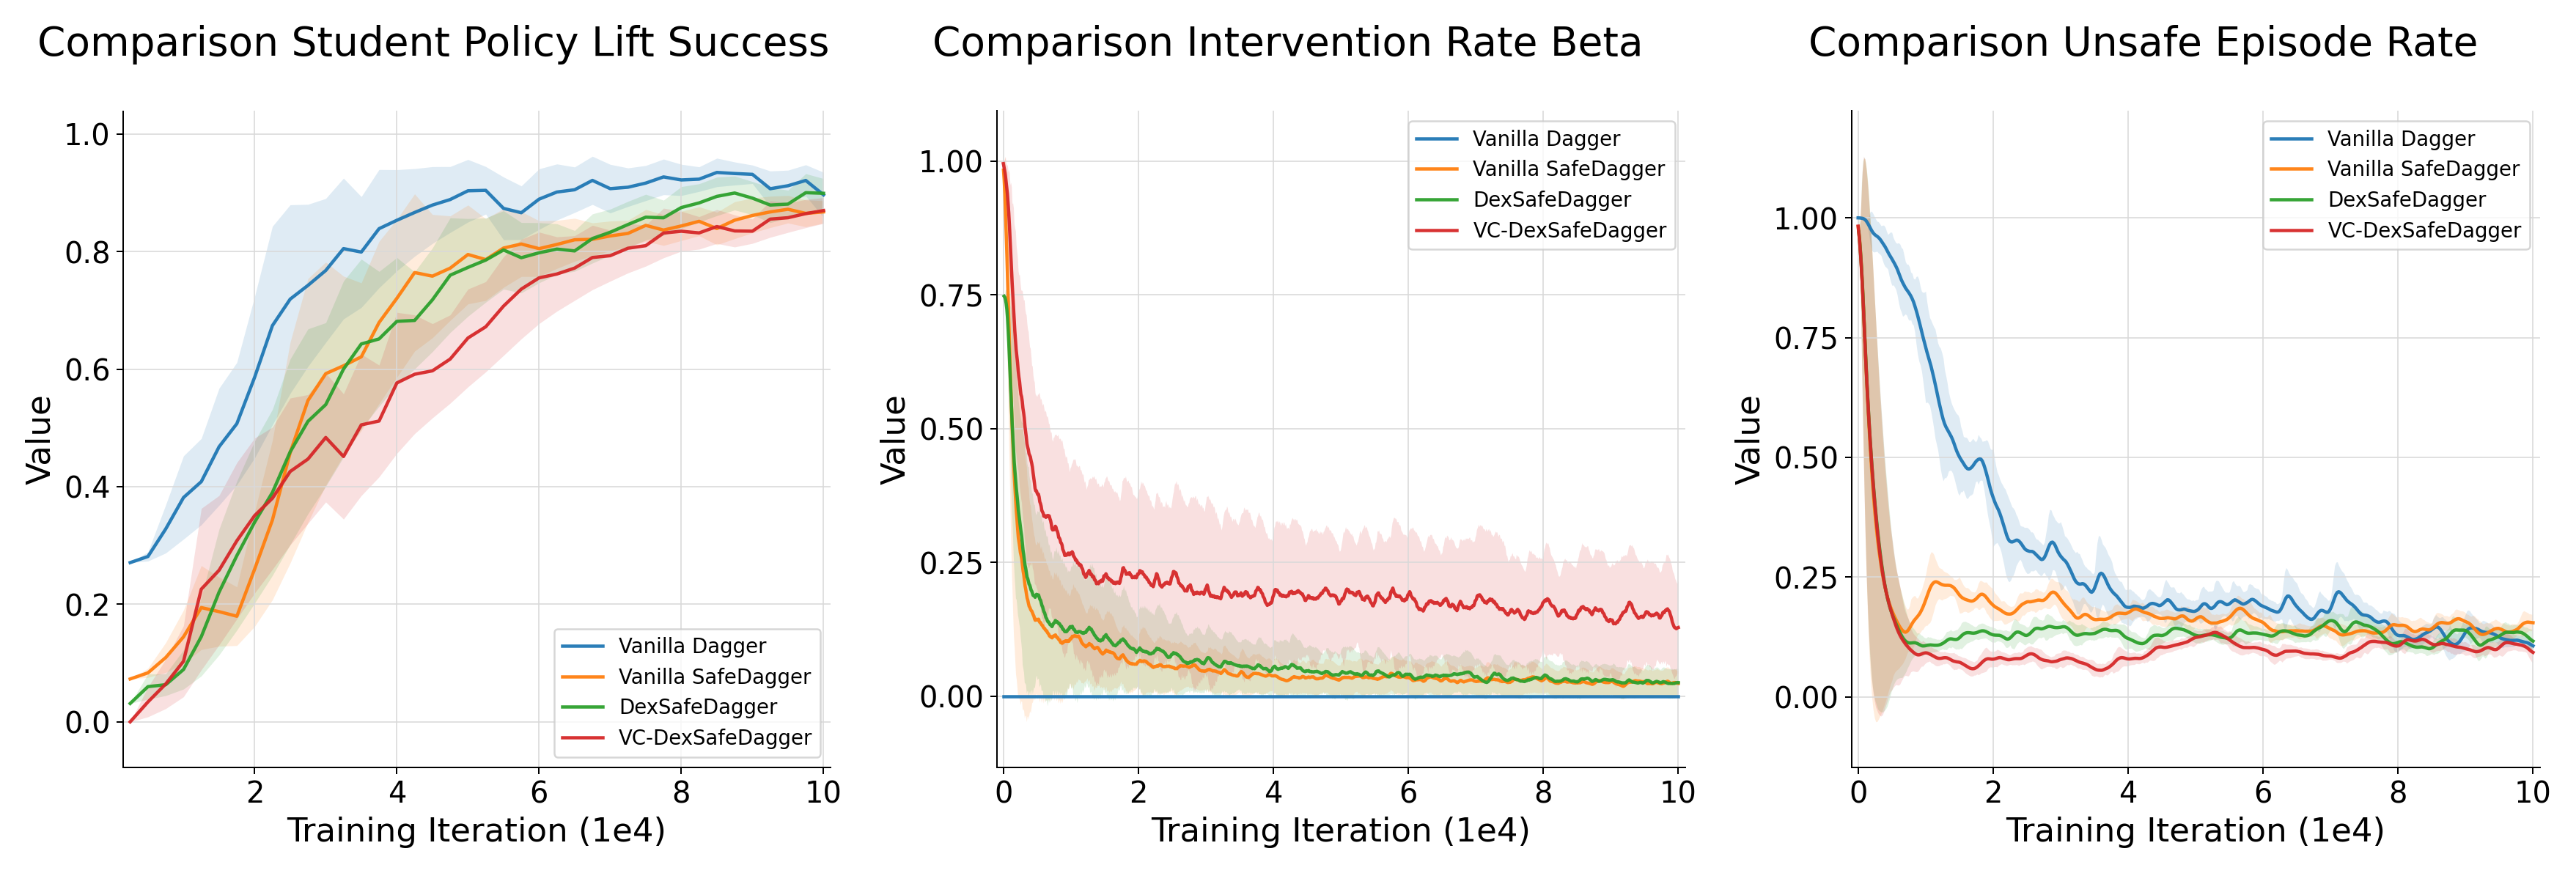
\includegraphics[width=\linewidth]{figures/ablation_comparison.png}
    \caption{\textbf{Ablation studies.}
    The first three panels compare four distillation variants in terms of student lift success, teacher intervention rate $\beta$, and unsafe episode rate, respectively, all plotted over training iterations.
    The rightmost panel shows the VLM-guided trajectory of the intervention operating point over online training.
    Shaded regions indicate variability across runs (mean $\pm$ std).
    Curves correspond to vanilla DAgger (blue), vanilla SafeDAgger (orange),
    \dexsafedagger (green), and \methodname (red).}
    \label{fig:ablation}
\end{figure*}

% The simulation experiments are based on single-arm control of a Tiangong~2 Pro
% humanoid robot equipped with InspireHand RH56DfX dexterous hands. The action
% space is 13-dimensional, consisting of 7 DoF for the robotic arm and 6 DoF for
% the dexterous hand.

% The student policy additionally receives image streams from two cameras at a
% resolution of $320\times240$ pixels and $30$\,fps. The raw stereo images are
% encoded by a visual encoder into a 64-D embedding, which is appended to the
% teacher actor observations to form the student observation. Concretely, the
% visual encoder uses a shared (Siamese) ResNet-18 backbone (last two layers
% removed) for each view, followed by an MLP projection and a 2-layer
% cross-attention transformer to fuse the two views; the resulting
% token is mapped to the 128-dimensional visual feature vector.

% Both teacher policy training and student skill distillation are conducted in Isaac Sim 5.0.0 and
% Isaac Lab 2.2.1 on a single NVIDIA RTX~5090 GPU.

% Forty objects sourced from the Omniverse Asset Library are tested in total. Each teacher policy is trained for 12{,}000 episodes,
% requiring approximately 3.5~hours. The teacher policies achieve a lift success rate ranging from 68\% to 
% 100\% and an unsafe rate ranging from 5\% to 30\%. The results are reported in Table~3.

% During student skill distillation, lighting intensity, direction and background textures are randomized at the
% beginning of each episode. Furthermore, object material properties, textures, and table appearance are randomized to encourage
% improved sim-to-real transfer, following a setup similar to DexTrAH-RGB. The distillation phase requires approximately 2.5~hours to complete
% 100{,}000 episodes.

Simulation experiments use single-arm control on a Tiangong~2 Pro humanoid equipped with InspireHand RH56DfX; the action
space is 13-D (7 arm DoF + 6 hand DoF). The RGB student additionally receives two $320\times240$ camera streams at
30\,fps, encoded by a Siamese ResNet-18 visual backbone with view fusion into a 128-D feature appended to the actor
observation. Teacher training and student distillation are conducted in Isaac Sim 5.0.0 / Isaac Lab 2.2.1 on a single
RTX~5090 GPU.

We evaluate 40 objects from the Omniverse Asset Library and train one
object-specific teacher for each object. Each teacher is trained for
12{,}000 episodes (3.5\,h), totaling 480{,}000 teacher-training
episodes and approximately 140 GPU-hours. Across the 40 teachers, lift-success
rates range from 72--100\%, and unsafe rates range from 5--30\%;
Table~\ref{tab:teacher_perf_200} reports a representative four-object subset.
During distillation, we randomize lighting intensity, direction, background
textures, object material, and table appearance following DexTrAH-RGB-style
domain randomization. The joint student is distilled across all 40 objects for
100{,}000 episodes in 2.5\,h. 

We use GPT-5.5 with high reasoning effort as the VLM. We issue the first VLM
query after 2{,}000 episodes
and subsequently query it every 10{,}000 distillation episodes, resulting in 10
VLM calls over the full 100{,}000-episode training run and approximately
70{,}000 tokens of total usage per run.

% \begin{table}[t]
\centering
\small
\caption{Observation spaces used for teacher RL training under the
asymmetric actor--critic framework.}
\label{tab:teacher_obs}
\resizebox{0.38\textwidth}{!}{%
\begin{tabular}{lcc}
\hline
\textbf{Observation Component} & \textbf{Actor} & \textbf{Critic} \\
\hline
Robot DOF positions  & 13 (noisy) & 13 \\
Robot DOF velocities  & 13 (noisy) & 13 \\
Hand link positions & 18 & 18 \\
Hand link velocities & 18 & 36 (twist) \\
Hand contact forces & -- & 3 \\
Measured joint torque & -- & 19 \\
Object position & 3 & 3 \\
Object rotation (quaternion) & 4 & 4 \\
Object velocity & -- & 6 (twist) \\
Goal position & 3 & 3 \\
Object scale & 1 & 1 \\
Previous actions & 13 & 13 \\
\hline
\textbf{Total dimension} & \textbf{86} & \textbf{132} \\
\hline
\end{tabular}
}
\end{table}

\begin{table}[t]
\centering
\small
\caption{Teacher policy performance on four representative objects from the
40-object training set (200 evaluation episodes per object).}
\label{tab:teacher_perf_200}
\setlength{\tabcolsep}{4pt}
\renewcommand{\arraystretch}{1.2}
\resizebox{0.38\textwidth}{!}{%

\begin{tabular}{l|cccc|c}
\hline
Metric (\%) & WindCart & Boot & ToolBox & Cow & \textbf{Mean} \\
\hline
Lift Success         & 93.5 & 100.0 & 88.5 & 87.0 & 92.3 \\
Unsafe Rate Avg      & 6.5   & 13.5  & 13.5 & 13.5 & 11.8 \\
Harmful collision    & 0.0   & 0.0   & 6.5  & 0.0  & 1.6  \\
Object escape        & 6.5   & 6.5   & 6.5  & 13.5 & 8.3  \\
Palm flipped         & 0.0   & 6.5   & 0.0  & 0.0  & 1.6  \\
Hand too far         & 0.0   & 0.0   & 0.0  & 0.0  & 0.0  \\
\hline
\end{tabular}
}
\end{table}


\subsection{Ablation Studies}

We perform the following ablation studies to validate the design choices in
\methodname and answer four questions: \textbf{(i)~Does our customized RL
recipe produce stronger teachers than the DexTrAH-RGB-style training recipe?}
\textbf{(ii)~Does the intervention mechanism in \dexsafedagger enable safer
exploration during policy distillation?} \textbf{(iii)~Does augmenting action
disagreement with success-value prediction improve the intervention signal?}
\textbf{(iv)~Is visual-language reasoning necessary for adapting the
intervention boundary?}

% \noindent\textbf{(a) DexTrAH-RGB RL teacher + Vanilla DAgger.}
% We follow the DexTrAH-RGB teacher training setup and distill the resulting teacher into a student using
% Vanilla DAgger. Rollouts in simulation are fully controlled by the student policy, while the teacher runs
% in parallel in the background with the intervention rate $\beta$ fixed to $0$. At each timestep, the
% executed student action $a_t^{S}$ is relabeled with the corresponding teacher action $a_t^{T}$.

\noindent\textbf{(a) DexTrAH-RGB RL + Vanilla DAgger.}
The teacher is trained using the DexTrAH-RGB RL recipe and then distilled into
a student policy using supervision only, with no teacher intervention during
rollouts ($\beta=0$).

% \noindent\textbf{(b) Our RL teacher + Vanilla DAgger.}
% We replace the DexTrAH-RGB teacher training pipeline with our customized RL recipe and use the same
% Vanilla DAgger-style online distillation.

\noindent\textbf{(b) Our RL + Vanilla DAgger.}
This setting matches (a), except that our RL recipe replaces the DexTrAH-RGB
teacher-training recipe.

% \noindent\textbf{(c) Our RL teacher + Vanilla SafeDAgger.}
% The teacher policy is trained using our RL pipeline, and we extend Vanilla DAgger to a Vanilla SafeDAgger
% distillation setup. The student and teacher policies are rolled out in parallel, and the teacher action takes
% over only when the $\ell_2$ distance between the teacher and student actions exceeds a threshold, indicating
% a large teacher--student disagreement. The student is trained on teacher-labeled pairs $(o_t^{S}, a_t^{T})$,
% where $o_t^{S}$ denotes the student observation.

\noindent\textbf{(c) Our RL + Vanilla SafeDAgger.}
The teacher training follows the recipe in (b), but we replace Vanilla DAgger
with a disagreement-gated SafeDAgger baseline. The teacher intervenes only when
$\lVert a_t^{T}-a_t^{S}\rVert_2$ exceeds a fixed threshold.

% \noindent\textbf{(d) DexTrAH-RGB RL teacher + SafeDAgger with disagreement and a success-value critic.}
% We follow the DexTrAH-RGB teacher training setup but apply our teacher-intervened distillation pipeline for
% student learning. The teacher and student policies are rolled out in parallel. Teacher intervention is triggered
% when either (i) the teacher disagrees with the student or (ii) the success-value critic flags the current transition
% as unlikely to lead to task success. The intervention decision is computed at every timestep. Likewise, the
% student is trained on teacher-labeled pairs $(o_t^{S}, a_t^{T})$.

\noindent\textbf{(d) DexTrAH-RGB RL + \dexsafedagger.}
We use the teacher-training recipe from (a) and the intervention baseline from
(c), extending it with a Bellman success-value critic under a stationary
intervention policy. Teacher intervention is triggered by either large
teacher--student disagreement or low predicted success.

% \noindent\textbf{(e) Our RL teacher + SafeDAgger with disagreement and a success-value critic.}
% We combine our custom RL pipeline with the proposed teacher intervention mechanism, using both teacher--student
% disagreement and success-value prediction to trigger teacher takeover.

\noindent\textbf{(e) Our RL + \dexsafedagger.}
Following the recipe in (d), we replace the teacher-training pipeline with our
customized RL recipe.

\noindent\textbf{(f) Our RL + \methodname.}
This setting extends (e) by replacing the stationary intervention policy with
the proposed VLM tuner, which periodically calibrates the disagreement-risk
intervention policy using rollout statistics and representative visual states.

\noindent\textbf{(g) Our RL + LLM-DexSafeDagger.}
This setting matches (f), except that the language model receives only the
rollout statistics and no visual observations.

\noindent\textbf{(h) Our RL + Grid-Search \dexsafedagger.}
This setting replaces the language/vision model in (f) with grid search over
the intervention thresholds. The remaining teacher, student, success-value
critic, and distillation components are held fixed.

To answer question~(i), we compare (a) with (b) and (d) with (e). The
DexTrAH-RGB-style RL recipe achieves lower performance than our RL recipe. We
attribute this gap to the specialized tuning of the \textsc{Fabrics} controller
for the original task setup, which transfers poorly to new hardware and
dynamics.

\begin{table}[t]
\centering
\small
\caption{Performance of ablations (a)--(h) on four representative objects from the
40-object training set (200 evaluation episodes per object). Each ablation
reports lift success and average unsafe rate.}
\label{tab:ablation_studies}
\setlength{\tabcolsep}{3pt}
\renewcommand{\arraystretch}{1.15}
\resizebox{0.48\textwidth}{!}{%
\begin{tabular}{l|cc|cc|cc|cc|cc}
\hline
\multirow{2}{*}{Metric (\%)}
& \multicolumn{2}{c|}{WindCart}
& \multicolumn{2}{c|}{Boot}
& \multicolumn{2}{c|}{ToolBox}
& \multicolumn{2}{c|}{Cow}
& \multicolumn{2}{c}{\revisionadded{\textbf{Mean}}} \\
\cline{2-11}
& Lift  & Unsafe
& Lift  & Unsafe
& Lift  & Unsafe
& Lift  & Unsafe
& \revisionadded{Lift}  & \revisionadded{Unsafe}  \\
\hline
\textbf{(a)} & 75.0 & 24.0 & 76.5 & 28.0 & 72.0 & 26.0 & 70.0 & 27.5 & \revisionadded{72.7} & \revisionadded{26.5} \\
\textbf{(b)} & 88.5 & 13.5 & 89.0 & 20.5 & 82.5 & 19.0 & 88.0 & 17.5 & \revisionadded{87.1} & \revisionadded{17.4} \\
\textbf{(c)} & 88.0 & 12.0 & 89.5 & 19.5 & 81.5 & 18.5 & 87.0 & 16.0 & \revisionadded{86.3} & \revisionadded{16.7} \\
\textbf{(d)} & 74.5 & 23.0 & 75.0 & 27.5 & 70.5 & 26.5 & 69.5 & 27.0 & \revisionadded{72.3} & \revisionadded{25.8} \\
\textbf{(e)} & 88.0 & 7.5 & 90.0 & 15.0 & 82.0 & 15.5 & 88.0 & 12.0 & \revisionadded{86.8} & \revisionadded{11.9} \\
\textbf{(f)} & 88.5 & 6.0 & 90.0 & 10.5 & 82.5 & 11.0 & 88.5 & 8.5 & \revisionadded{87.5} & \revisionadded{9.3} \\
\revisionadded{\textbf{(g)}} & \revisionadded{88.0} & \revisionadded{7.5} & \revisionadded{89.5} & \revisionadded{12.5} & \revisionadded{82.0} & \revisionadded{13.0} & \revisionadded{88.0} & \revisionadded{10.5} & \revisionadded{86.9} & \revisionadded{10.2} \\
\revisionadded{\textbf{(h)}} & \revisionadded{86.5} & \revisionadded{7.0} & \revisionadded{88.5} & \revisionadded{14.0} & \revisionadded{81.0} & \revisionadded{13.5} & \revisionadded{87.0} & \revisionadded{11.0} & \revisionadded{85.7} & \revisionadded{11.7} \\
\hline
\end{tabular}
}
\end{table}


\begin{figure*}[!t]
    \centering
    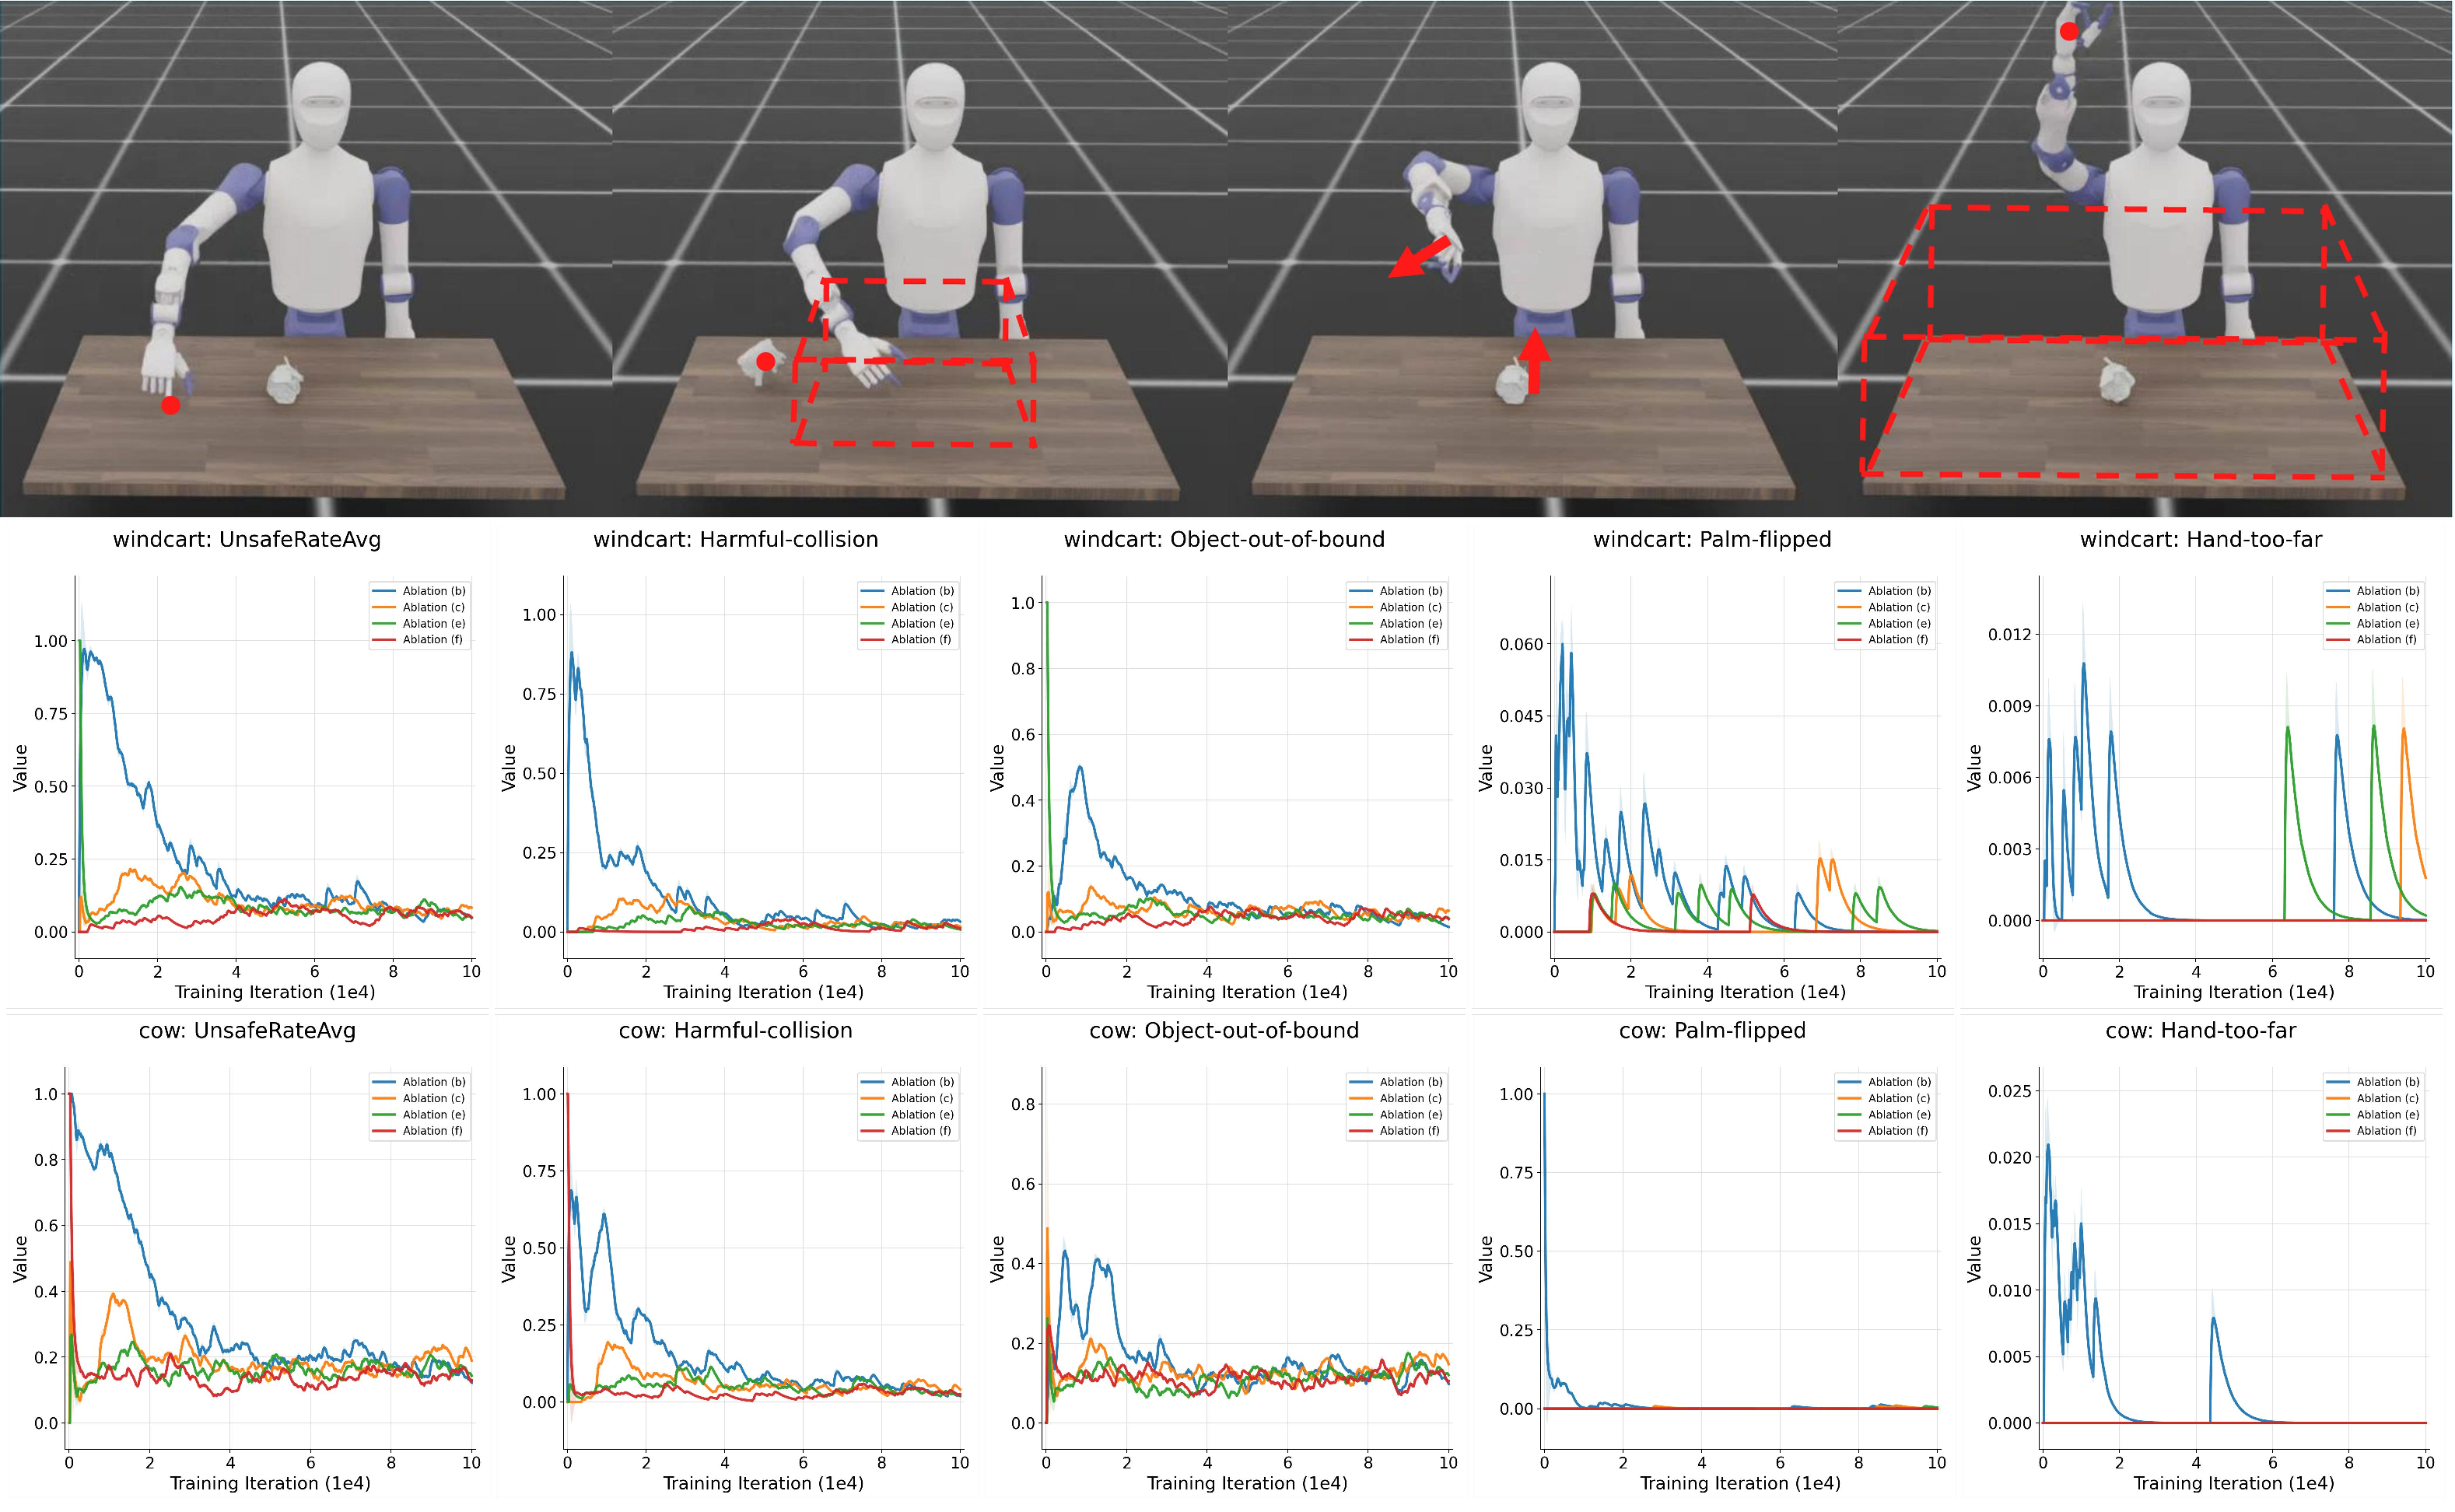
\includegraphics[width=0.82\linewidth]{figures/failure_mode.pdf}
    \caption{\textbf{Per-object failure-mode decomposition during online distillation ablations.}
    We illustrate four task-specific failure modes in simulation (harmful collision, object escape, palm flipped, and hand too far) and report the aggregate unsafe rate together with its per-mode breakdown over training iterations.
    Results are shown for two objects (\texttt{windcart} and \texttt{cow}); lower is better in all plots.
    Curves correspond to four distillation variants: blue, Vanilla DAgger\cite{ross2011reduction};
    orange, Vanilla SafeDAgger\cite{zhang2016query}; green, \dexsafedagger;
    and red, \methodname.}
    \label{fig:failure_modes}
\end{figure*}

We next address question~(ii) by examining the distillation behavior in
Fig.~\ref{fig:ablation}. Ablations (b), (c),
(e), and (f) achieve comparable final lift success
(left), consistent with the intervention policy's focus on safety rather than task success. Unlike
Vanilla DAgger ($\beta=0$), the three intervention variants reduce teacher intervention as the student
improves (middle). They reduce early unsafe episodes by approximately 80\% relative to Vanilla DAgger and
remain below 20\% throughout distillation, with \methodname achieving the lowest rate overall (right).

We address question~(iii) by comparing ablation (c), which uses disagreement alone,
with ablation (e), which adds success-value prediction
while retaining the same RL teacher and stationary intervention policy. The combined gate
intervenes in low-predicted-success states missed by disagreement alone, reducing the average
unsafe-episode rate by about 7.5 percentage points and limiting collision and object-escape
failures without sacrificing task performance. Its unsafe rate approaches the teacher's
average ($\approx 12\%$) by the end of training and reaches a minimum of approximately 8\%.
Fig.~\ref{fig:failure_modes} further shows that harmful collisions and object
escape dominate unsafe episodes. Compared with Vanilla DAgger, all three
intervention variants suppress both failure modes, particularly their early
spikes, demonstrating that teacher intervention limits unsafe exploration
during the initial distillation phase.

\begin{figure}[!t]
    \centering
    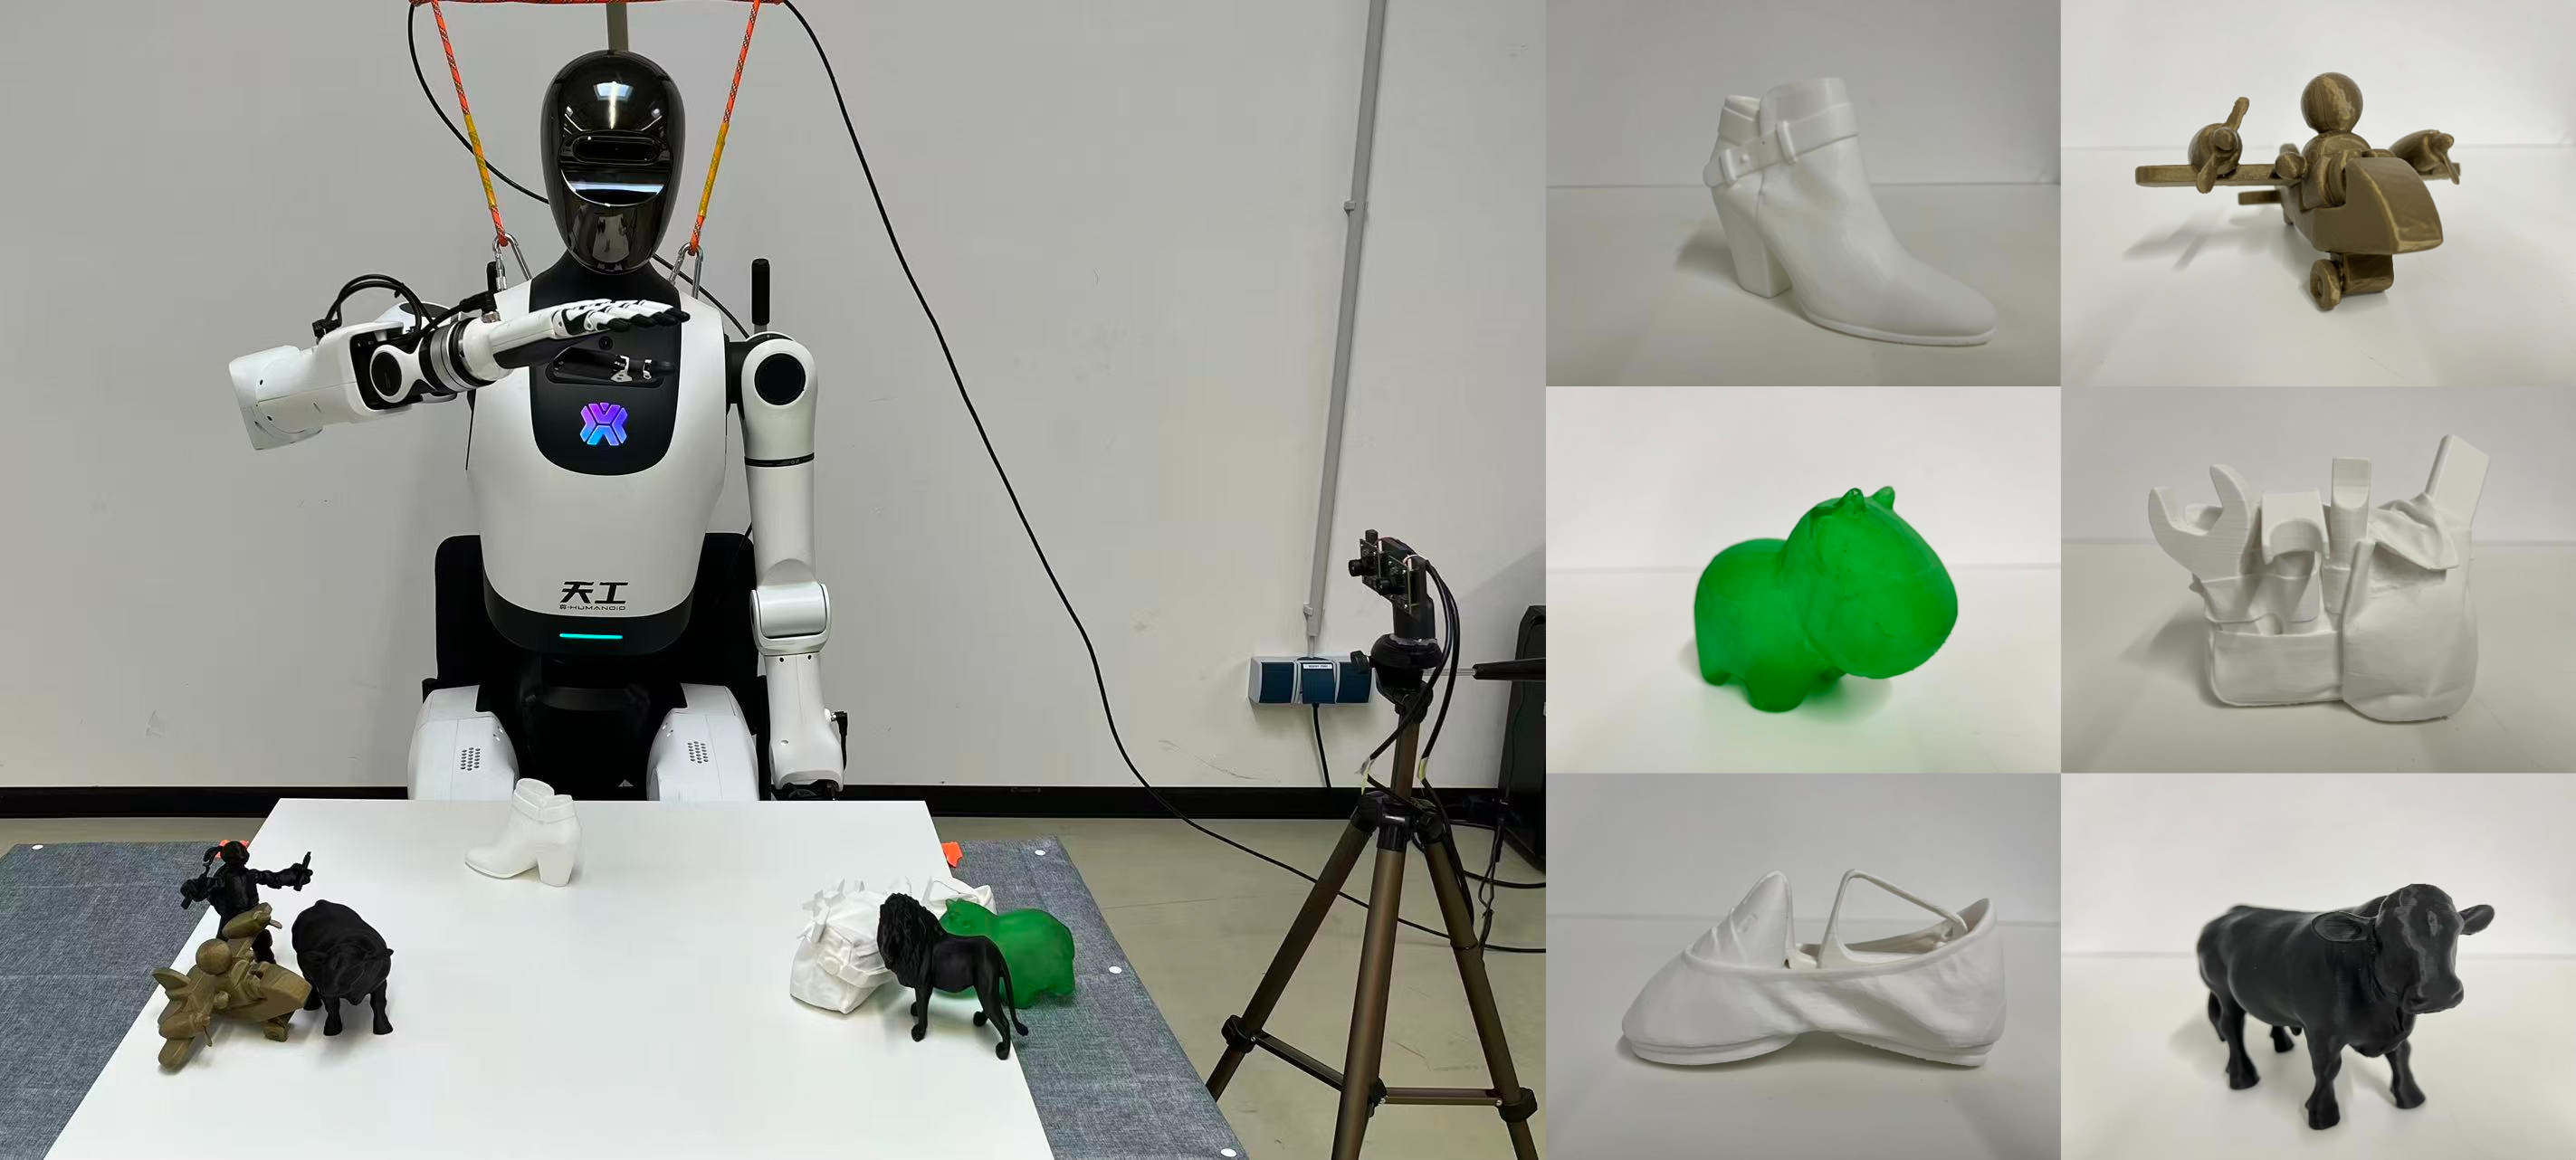
\includegraphics[width=0.85\linewidth]{figures/real_setup_1.png}
    \caption{\textbf{Real-world experimental setup and test objects.}
    Left: the single-arm manipulation platform used for deployment and evaluation.
    Right: examples of the physical objects used in the real-world lift experiments.}
    \label{fig:realworld_exp_setup}
\end{figure}

Finally, we address question~(iv) by comparing ablations (e), (h), (g), and
(f), which form a progression from stationary intervention, to grid-searched
thresholds, to semantics-guided LLM adaptation, and finally to our VLM-guided
recipe. This controlled ladder isolates the contributions of threshold
adaptation, semantic reasoning, and visual context.
\textcolor{red}{TODO: Add the quantitative comparison of ablations (e), (h),
(g), and (f) when the evaluation results are available.}
Across all evaluated
objects, ablation (f) achieves an unsafe-episode rate that is lower than that
of (e) by an average of 4 percentage points, while maintaining comparable lift
success. This result shows that VLM-guided intervention-policy adaptation
improves safety without sacrificing task performance.

\subsection{Real-World Experimental Results}

We evaluate the deployed student policy on 22 objects, comprising 16 seen objects and 6 unseen objects.
Table~\ref{tab:real_world_results} reports a representative six-object subset
and pooled results for the four seen and two unseen objects shown.
The experiments exhibit a lower lift success rate and a higher unsafe episode rate than
the teacher and student evaluation results in simulation, indicating that \methodname does
not fully eliminate the sim-to-real gap. Nevertheless, the resulting policy is sufficiently robust
for real-world deployment.

The unseen-object evaluation reveals a clear generalization gap: compared with
the seen objects shown, the policy's pooled lift success decreases from
\textcolor{red}{85.0\%} to \textcolor{red}{63.3\%}, while its unsafe rate
increases from \textcolor{red}{20.0\%} to \textcolor{red}{40.0\%} on the unseen
objects shown. This degradation is
primarily driven by increased harmful collisions (20.0\% and 26.7\% on Plane and
Shoe), while object escape remains comparable across objects
($\approx$6.7--20.0\%). No palm-flip or hand-too-far events are observed,
suggesting that real-world failures are dominated by contact-rich interactions
rather than gross pose instabilities. Overall, the results indicate that the
remaining sim-to-real gap on unseen geometries is largely attributable to a
contact-strategy mismatch, i.e., the policy fails to adapt its contact
interactions to novel object shapes.

\newcommand{\unseen}[1]{\cellcolor{gray!15}\textbf{#1}}

\begin{table}[t]
\centering
\small
\caption{Representative six-object subset of the 22-object real-world evaluation
(30 episodes per object). The last two columns report pooled results over the
complete sets of 16 seen and 6 unseen objects, respectively. \unseen{Unseen
objects} are shaded.}
\label{tab:real_world_results}
\setlength{\tabcolsep}{4pt}
\renewcommand{\arraystretch}{1.2}
\resizebox{0.48\textwidth}{!}{%

\begin{tabular}{l|cccccc|cc}
\hline
Metric (\%) & WindCart & Boot & ToolBox & Cow & \unseen{Plane} & \unseen{Shoe}
& \makecell{{\textbf{Seen}} \\ {\textbf{avg. (16)}}}
& \unseen{{\makecell{Unseen \\ avg. (6)}}} \\
\hline
Lift Success         & 87.0 & 86.3 & 80.0 & 86.7 & \unseen{66.7} & \unseen{60.0} & 86.2 & \unseen{63.9} \\
Unsafe Rate Avg      & 13.3 & 19.7 & 20.0 & 25.7 & \unseen{40.0} & \unseen{40.0} & 21.2 & \unseen{34.8} \\
Harmful collision    & 0.0  & 6.7  & 13.0 & 13.3 & \unseen{20.0} & \unseen{26.7} & 9.3  & \unseen{20.1} \\
Object escape        & 13.3 & 13.0 & 7.0  & 12.7 & \unseen{20.0} & \unseen{13.3} & 11.9 & \unseen{13.8} \\
Palm flipped         & 0.0  & 0.0  & 0.0  & 0.0  & \unseen{0.0}  & \unseen{0.0}  & 0.0 & \unseen{0.2}  \\
Hand too far         & 0.0  & 0.0  & 0.0  & 0.0  & \unseen{0.0}  & \unseen{0.0}  & 0.0  & \unseen{0.7}  \\
\hline
\end{tabular}
}
\end{table}


% \subsection{Discussion}

% While effectively reducing unsafe exploration, the teacher-intervened online distillation process
% appears to reduce sample efficiency. In Fig.~\ref{fig:ablation}, we observe slower performance growth in
% lift-success evaluation under higher intervention rates. The underlying cause remains unclear; we believe
% there is room for improvement in both exploration safety and sample efficiency within the online
% distillation paradigm.
